\documentclass[tikz,border=5pt]{standalone}
\usepackage{amsmath,amssymb}
\usepackage{tikz}
\begin{document}
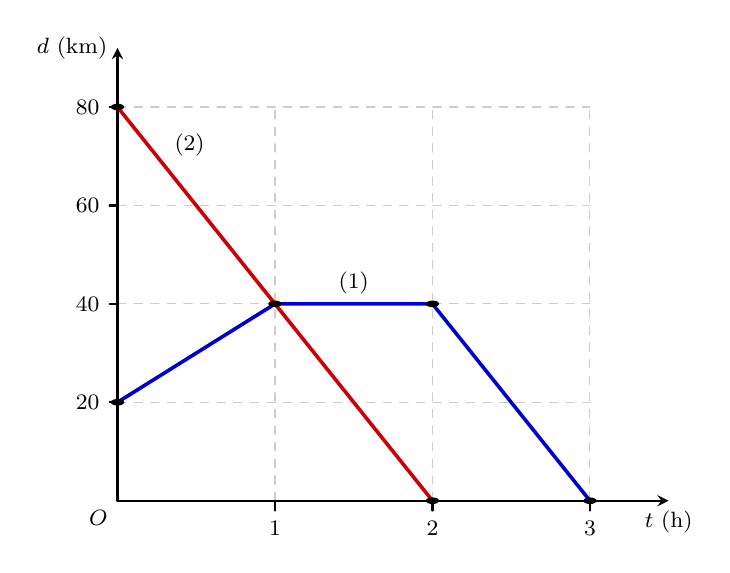
\begin{tikzpicture}[>=stealth, line join=round, line cap=round, font=\footnotesize, xscale=2, yscale=0.0625]
	% Lưới tọa độ
	\foreach \x in {1, 2, 3} {
		\draw[dashed, gray!40, thin] (\x, 0) -- (\x, 80);
	}
	\foreach \y in {20, 40, 60, 80} {
		\draw[dashed, gray!40, thin] (0, \y) -- (3, \y);
	}
	% Trục tọa độ
	\draw[->, thick] (0, 0) -- (3.5, 0) node[below] {$t\text{ (h)}$};
	\draw[->, thick] (0, 0) -- (0, 92) node[left] {$d\text{ (km)}$};
	\node[below left] at (0, 0) {$O$};
	
	% Vạch chia
	\foreach \x in {1, 2, 3} {
		\draw[thick] (\x, 0) -- (\x, -2) node[below] {$\x$};
	}
	\foreach \y in {20, 40, 60, 80} {
		\draw[thick] (0, \y) -- (-0.05, \y) node[left] {$\y$};
	}
	
	% Đường (1): từ (0; 20) -> (1; 40) -> (2; 40) -> (3; 0)
	\draw[line width=1.3pt, blue!80!black] (0, 20) -- (1, 40) -- (2, 40) -- (3, 0);
	\node[above] at (1.5, 40) {$(1)$};
	
	% Đường (2): từ (0; 80) -> (2; 0)
	\draw[line width=1.3pt, red!80!black] (0, 80) -- (2, 0);
	\node[above right] at (0.3, 68) {$(2)$};
	
	\foreach \p in {(0,20), (1,40), (2,40), (3,0), (0,80), (2,0)} {
		\fill[black] \p circle (1.2pt and 19pt);
	}
\end{tikzpicture}
\end{document}
